\documentclass{article}

\usepackage[utf8]{inputenc}
\usepackage{tikz}
\usepackage{siunitx}
\usepackage{amsmath,amsthm}

\newcommand{\deriv}[2]{\frac{\mathrm{d}#1}{\mathrm{d}#2}}
\newcommand{\pderiv}[2]{\frac{\partial#1}{\partial#2}}
\newcommand{\ii}{\mathbf{i}}

\bibliographystyle{unsrt}

% siunitx stuff
\newunit{\byte}{B}
\newprefix[binary]{\kibi}{10}{ki}
\newprefix[binary]{\mebi}{20}{Mi}
\newprefix[binary]{\gibi}{30}{Gi}

\newtheorem{theorem}{Theorem}[section]
\theoremstyle{definition}
\newtheorem{definition}{Definition}

\author{Matthew Cox\\250233041}
\date{\today}
\title{The Distributed Discrete Fourier Transform}

\begin{document}
\maketitle

\tableofcontents

\section{Motivation}
In the analysis of magnetic materials, models consisting of dipoles on a lattice
interacting by a variety of electromagnetically-mediated interactions occur
ubiquitously. This general class of models is very flexible because there is a
great variety in how the interactions between the dipoles are treated. These
interactions may be loosely classified as follows:

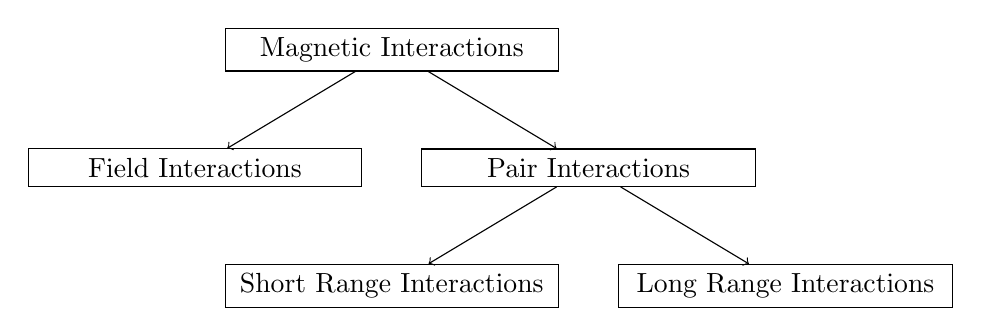
\begin{tikzpicture}[
  class/.style={rectangle, draw, text centered,text width=4cm},
  space/.style={sibling distance=5cm}
  ]

  \node[class] {Magnetic Interactions} [space,->]
    child { node[class] {Field Interactions} }
    child { node[class] {Pair Interactions} [space]
      child { node[class] {Short Range Interactions} }
      child { node[class] {Long Range Interactions} }
    };
\end{tikzpicture}

The interactions between individual particles and a field extrinsic to the
remaining particles are trivial to simulate, we have termed these \emph{field
interactions} in the above diagram. Sources which may give rise to interactions
form are anisotropy in the lattice and externally applied fields. The
interactions between particles on the lattice are more complicated to simulate,
and they are classified into short and long range interactions. These names
reflect their geometry, but they also reflect a fundamental difference in
computational complexity encountered their simulation.

The objective of simulation in material physics is to understand macroscopic and
mesoscopic phenomena, but our models are defined in terms of microscopic
components. This difference in scale leads to the first difficulty we encounter
in simulation: to obtain meaningful results, our simulations must be of vast
scales. The spacing of individual atoms is on the order of
\SI{1e-10}{\meter}, while the typical macroscopic scale we are interested is of
no less than \SI{1e-3}{m}. For a three dimensional lattice, we must simulate
some \num{1e21} particles, a computationally intractable task. (For spins
represented by three IEEE-754 double precision integers, we would require some
\SI{2.24e13}{\gibi\byte} of storage to represent the configuration.) We might
naïvely believe that if we are only interested in mesoscopic dynamics, such a
large lattice is not required and the problem of an impossibly large lattice is
avoided. To the contrary, a simulation on a small finite lattice is subject to
\emph{edge effects,} which arise because the dipoles near the edge experience a
different environment than the centrally situated dipoles---edge particles
interact with fewer particles at some given distance, and their interacting
partners are asymmetrically distributed in space.

To avoid edge effects and the need to simulate vast lattices, we simulate a
finite lattice and introduce periodic boundary conditions. The simulated lattice
is repeated in all directions, each repetition is termed a cell, and the
repeated spins are termed replicas. This eliminates edge effects, but if the
lattice is chosen to be too small, there may still be simulation artifacts due
to \emph{self-image} interactions. These arise when a prominent feature
interacts with its own replica: the periodic lattice introduces a sort of
resonance which tends to produce artifacts which have a wavelength dividing the
lattice size. To avoid this, we need to ensure that dipoles are well separated
from their replicas, and thus the lattice size needs to be large relative to the
effective range of the longest range interaction in the system.

In order to handle the large lattices necessary for accurate and meaningful
simulation, there are two reasons to consider distributed simulation. Firstly,
the large number of dipoles in the simulation require a correspondingly large
amount of computation to advance the simulation. (We will discuss the actual
asymptotic complexity in the next section.) Secondly, we may simulate lattices
too large to fit in a single computer's memory by distributing it across a
cluster of processors.


In the next section, we will examine the Landau-Lifshitz-Gilbert model for the
evolution of a dipole in a magnetic field, and how the interaction of particles
dictates the structure of a distributed simulation. We will then show how to
efficiently compute the long range interaction by means of Ewald summation. The
remainder of the work will discuss our implementation of the distributed
discrete Fourier transform.

\section{The Landau-Lifshitz-Gilbert Model}

Our interest lies in thin magnetic films, which one may think of as an infinite
plane of interacting dipoles in a lattice. These find physical application in
various sensors and computer storage systems, and our eventual goal is the study
of mesoscopic phenomena in thin magnetic films. The starting point for our
modelling is the Landau-Lifshitz-Gilbert equation, obtained by Gilbert from an
original model by Landau and Lifshitz by correcting the damping term for a
larger range of damping coefficients\cite{gilbertLLG}. Representing the
orientation of a dipole by its orientation and magnitude as a three-vector
$\sigma$, we have:
\begin{equation}\label{eqn:LLG}
  -\deriv{\sigma}{t} = \frac{\gamma}{1 + \alpha^2} \sigma \times H +
\frac{\gamma \alpha}{1 + \alpha^2} \sigma \times (\sigma \times H)
\end{equation}
where $H$ denotes the magnetic field at the dipole's location. The first term of
the right side of the equation describes the precession of the spin about a
magnetic field, while the second is a damping term which causes the relaxation
of the spin towards a stable configuration (aligned to to the field and pointing
in the opposite direction). The particular form of $H$ is derived from physical
considerations. To incorporate thermal effects into our model, we write $H$ as
the sum of a deterministic component $H_\text{det}$ and a Langevin term
$H_\text{lan}$ which is a vector of independent Guassian stochastic variables
with zero mean and some temperature dependent variance. (The correct variance may be
obtained by the fluctuation-dissipation relation.) This creates an Itô
stochastic differential equation, and the numeric integration procedure must be
consistent with the definition of the Itô integral.

\begin{figure}
\caption{\label{fig:lattice1} Schematic of Spin Interaction Geometry. The green
and red lines represent (respectively) the effective range of the long and short
range interparticle interactions. The numbered nodes contribute to the short
range field at site $i$. The spin at site $j$ interacts via the dipole
interaction with the displacement vector $r_{ij}$ as indicated.}
\begin{center}
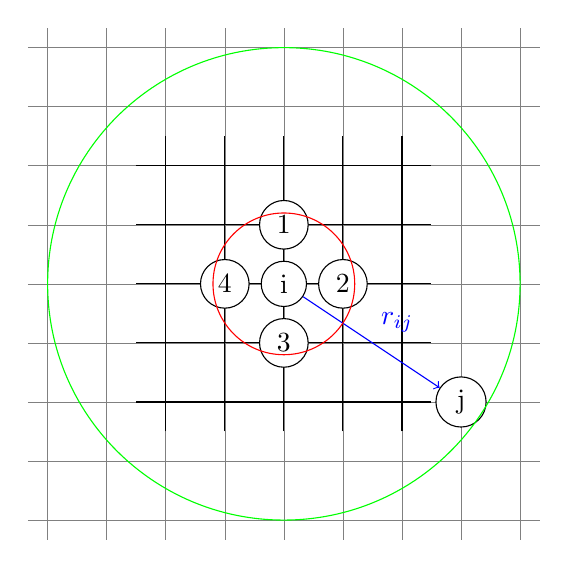
\begin{tikzpicture}[
  replica/.style={very thin,color=gray},
  spin/.style={circle,fill=white,draw=black}
]
  \draw[replica,step=0.75cm] (-3.25cm,-3.25cm) grid (3.25cm,3.25cm);
  \draw[step=0.75cm] (-1.875cm,-1.875cm) grid (1.875cm, 1.875cm);
  \draw (0,0) node[spin] (i) {i}
        (2.25,-1.5) node[spin] (j) {j}
        (0,0.75) node[spin] {1}
        (0.75,0) node[spin] {2}
        (0,-0.75) node[spin] {3}
        (-0.75,0) node[spin] {4};
  \draw[->,blue,auto] (i) to node {$r_{ij}$} (j);
  \draw[red] (i) circle (0.9cm);
  \draw[green] (i) circle (3cm);
\end{tikzpicture}\end{center}
\end{figure}


The deterministic term itself is understood to consist of three terms which
comprise the field, short range, and long range interactions. The field
interactions are computed as a function of the spin index, and there is no
particular difficulty in a distributed implementation. To analyze the
interaction of two spins, consider the multipole expansion of the field of some
spin. Since each dipole is electrically neutral, there is no monopole field, and
the leading (and longest range) interaction is the dipole interaction. The
expression for the field at the $i$-th lattice site due to the charge at the
$j$-th lattice site is given by:
\begin{displaymath}
  H^\text{dipole}_{ij} = \frac{\sigma_j}{\|r_{ij}\|^3} - \frac{3 \langle
\sigma_j , r_{ij} \rangle r_{ij}}{\|r_{ij}\|^5}
\end{displaymath}
where $r_{ij}$ is the displacement vector from site $i$ to site $j$. (Note that
the field is unchanged under the replacement of $r_{ij}$ with $-r_{ij}$, and thus
there is no need to specify which of $i$ and $j$ is the origin and which the
terminus of the displacement vector.) The remaining higher order fields are
short ranged, and can be considered as part of the short range interaction.

The short range interaction occurs between adjacent lattice sites. The
functional dependence of the short range field at lattice site $i$ is upon those
sites $j$ which neighbour $i$. The lattice structure is regular, therefore each
spin has a constant number of neighbours (recall that the spins on the edge
interact with the periodic replicas of the spins on the opposite edge). We
conclude that the computational cost of the short field interaction is linear in
the number of spins. Figure \ref{fig:lattice1} demonstrates the interaction
geometry which we have hitherto described. The darker grid region in the center
is meant to represent the simulated lattice (the center cell), and the lighter
grid at the edge of the diagram represents spins which are periodic replicas of
the center cell. Notice that the long range dipole interaction includes
contributions from a replicated spin.

The geometry of the interactions dictates the distribution of the lattice in a
distributed simulation. The short range interaction involves the interaction
between neighbouring spins, this implies that neighbouring spins should be on
the same processor to minimize communication requirements. We see that the unit
cell should be partitioned into contiguous domains since no communication is
required to compute the short range interaction on the interior spins.
Communication with the processors managing neighbouring domains is required to
compute the short range interaction effecting the edge sites. To minimize the
communication costs, the edges should be as small as possible. We therefore
choose a ``checkerboard'' layout of the processors.

The long field interaction is costly to simulate. A given spin will interact
with every other particle in the grid (and its periodic replicas), therefore we
must consider the long field exchange between every single pair of particles.
This leads to a computational cost which is quadratic in the number of spins.
(The cost is not infinite as we have assumed that the interaction with all the
replicas of a given spin can be handled in one constant time operation.) The
much graver issue is that each processor must exchange its state with every
other processor, leading to a communication cost which is also quadratic in the
number of spins! This communication overhead is unacceptable on all but the most
expensive and specialized parallel systems, and so the naïve method of direct
summation will not lead to an efficient simulation algorithm. We must turn to a
more efficient numerical method for the evaluation of long range interactions.

\section{Ewald Summation}
The direct computation of the dipolar interaction requires a number of
computations proportional to the square of the number of spins, and (in a
distributed simulation) a quadratic cost in communication since each processor
needs to know the value of the dipoles stored on every other processor. Since
the dipole field needs to be recomputed at each simulation step, we can
significantly increase the performance of our simulation by finding an
asymptotically more efficient implementation. A method developed by Ewald is to
rewrite the sum of the particle fields as a convolution between the spins on the
lattice and the coupling tensors\cite{kittleSSP}. We can then apply the discrete
Fourier transform to compute the convolution efficiently in frequency space. The
fields can be recovered by inverting the Fourier transform. In this section, we
will derive the expression for the long range fields which is amenable to
computation by the Fourier transform.

We assume a two dimensional periodic lattice, each cell of which contains $M
\times N$ sites. We denote by $\sigma_{i,j}$ the spin at lattice coordinates
$(i,j)$, which is represented by a three dimensional vector with orientation and
spin corresponding to the orientation and magnitude of the dipole moment of the
spin. The field at lattice site $(i,j)$ due to the spin at $(i',j')$ is:
\begin{equation}
g \sigma^b \left( \frac{\delta_{\alpha,\beta}}{\| r \|^3} - 3 \frac{r^\alpha
r^\beta}{\| r \|^5} \right)
\end{equation}
Where we have adopted the Einstein summation convention, greek letters indicate
components of vectors, and denoted the displacement vector from $(i,j)$ to
$(i',j')$ by $r$. If we understand the quantity in brackets as an interaction
tensor, then by summing over all the repeated replicas, we obtain the expression
for the field at lattice site $(i,j)$:
\begin{equation}
H_{i,j}^\alpha = \sum_{m,n=-\infty}^{\infty} \sum_{i',j'=0}^{M,N}
\sigma_{i',j'}^\beta \gamma_{\alpha,\beta} \left( (i,j) - (i' + mM, j' + nN)
\right)
\end{equation}
Where we have defined the dipole interaction tensor:
\begin{displaymath}
\gamma_{\alpha,\beta}(r) = \begin{cases}
  0 & \text{if } r = 0 \\
  \frac{\delta_{\alpha,\beta}}{\| r \|^3} - 3 \frac{r^\alpha r^\beta}{\| r \|^5}
& \text{otherwise}
\end{cases}
\end{displaymath}
The $r = 0$ case corresponds to the impossible situation of a dipole interacting with
itself, thus we set the interaction tensor to zero in this case. This simplifies
the analysis by eliminating the need to specifically exclude self-interactions.
Notice that this does not exclude interactions between a particle and its
replica in another cell.

Returning to our expression for $H_{i,j}^\alpha$, we can take advantage of the
periodicity of the spins to rewrite the summation indices:
\begin{displaymath}
H_{i,j}^\alpha = \sum_{m,n=-\infty}^{\infty} \sum_{\substack{i' = i - M\\j' = j
- N}}^{i,j} \sigma_{i',j'}^\beta \gamma_{\alpha,\beta} \left( (i,j) - (i' + mM,
j' + nN) \right)
\end{displaymath}

Exchanging the variable $i'$ for $i - i'$ and similarly for $j'$ yields:
\begin{displaymath}
H_{i,j}^\alpha = \sum_{i',j' = 0}^{M,N}
\sigma_{i-i',j-j'}^\beta \left( \sum_{m,n=-\infty}^{\infty}
\gamma_{\alpha,\beta} \left(i' + mM, j' + nN \right) \right)
\end{displaymath}

The term in brackets represents the field due to a particle located at a
displacement $(i',j')$ and all of its periodic replicas. To evaluate the sum, we
can truncate the sum on the justification that for very large magnitudes of $m$
and $n$, the term vanishes. Another interpretation (and means to compute the
value) is as the convolution of the primitive solution $\gamma_{\alpha,\beta}$
with the lattice indicator function:
\begin{displaymath}
L_{i,j} = \sum_{m,n = -\infty}^\infty \delta((i - mM, j - nN))
\end{displaymath}
This is analogous to the solution of Poisson's equation by convolution of a
Greens function with the charge distribution. However it is computed, we define:
\begin{displaymath}
\Gamma_{\alpha,\beta}(r) = \sum_{m,n=-\infty}^{\infty} \gamma_{\alpha,\beta}
\left( r + (mM,nN) \right)
\end{displaymath}
And thus obtain the following convolution for the dipole field:
\begin{equation}\label{eqn:convLR}
H_{i,j}^\alpha = \sum_{i',j' = 0}^{M,N} \sigma_{i-i',j-j'}^\beta
\Gamma_{\alpha,\beta}\left((i',j')\right)
\end{equation}
This form still requires a quadratic amount of computation to evaluate as
written (there are $MN$ terms in the sum, and we need to evaluate it for $MN$
lattice locations). The discrete Fourier transform can be used to efficiently
compute the convolution, and in a distributed implementation also asymptotically
lowers the communication requirements.

It is worth noting that in three dimensions, the Ewald summation method yields a
conditionally convergent series. In fact, the summation of the dipole fields is
conditionally convergent by any means. The rough explanation of this phenomenon
is that the dipole interaction decays in magnetude proportional to $r^{-3}$,
while the number of particles at a given distance is proportional to $r^2$.
Therefore the magnitude of the field recieved from spins at some given distance
is proportional to $r^{-1}$, the summation over distance therefore yields a
conditionally convergent sequence. We can safely ignore this in our two
dimensional problem, since in two dimensions the number of interacting partners
scales with distance linearly, so the magnitude of the field from particles at
distance $r$ falls off with $r^{-2}$. This sum is absolutely convergent.

\section{The Discrete Fourier Transform}
The discrete Fourier transform is an analogue of the classical Fourier transform
defined for vectors of values which are uniformly distributed in time or space.
Like the classical Fourier transform, the discrete Fourier transform computes a
representation of the data in a basis of periodic components (more specifically,
in terms of the amplitudes and phases of periodic components).
\begin{definition}[The Discrete Fourier Transform\cite{walkerFFT}]
For an $N$-length finite sequence of complex numbers $\{x_n\}$, the discrete Fourier
transform of $\{x_n\}$ is an $N$-length finite sequence of complex numbers which
are defined by the following equation:
\begin{equation}\label{eqn:defDFT}
 \hat{x}_k = \sum_{n=0}^{N-1} x_n e^{-\frac{2 \pi \ii k n}{N}}
\end{equation}
\end{definition}

We have stated that the discrete Fourier transform is a mere change of basis
from the positional basis $\{\{1,0,0,0\dots\}, \{0,1,0,0\dots\},
\{0,0,1,0\dots\}\}$ to a periodic basis. Since all the sequences we will deal
with in this work are finite, this eliminates many subtle issues of convergence
and of representations within infinite dimensional spaces. One natural challenge
to this assertion that the discrete Fourier transform is a change of basis is to
demand the inverse transform. The following theorem shows that the inverse
discrete Fourier transform is very similar to \eqref{eqn:defDFT}.
\begin{theorem}[The Inverse Fourier Transform]
Let $\{\hat{x}_k\}$ be the discrete Fourier transform of $\{x_n\}$, a length $N$
sequence. The original sequence $\{x_n\}$ and the coordinates $\{\hat{x}_k\}$ of
the sequence in the length $N$ Fourier basis satisfy:
\begin{equation}\label{eqn:invDFT}
  x_n = \frac{1}{N} \sum_{k=0}^{N-1} \hat{x}_k e^{\frac{2 \pi \ii k n}{N}}
\end{equation}
\end{theorem}
\begin{proof}
Substitute \eqref{eqn:defDFT} into the right side of \eqref{eqn:invDFT} to
obtain:
\begin{displaymath}
  \frac{1}{N} \sum_{k=0}^{N-1} \sum_{m=0}^{N-1} x_m e^{-\frac{2 \pi \ii k (n -
m)}{N}}
\end{displaymath}
The summation with respect to $k$ is zero for all $m \not= n$. Suppose that $n -
m = pN + \alpha$ for some non-negative $\alpha$ less than $N$. Then the
exponential in the expression becomes $\exp ( - \frac{2\pi \ii k \alpha}{N} )$.
The summation over $k$ is a sum over $N$ values distributed uniformly on the
unit circle in the complex plane: the sum must be zero. (Recall that the center of
mass of equal point masses spaced evenly on the unit circle is the origin.) We
therefore obtain:
\begin{displaymath}
  \frac{1}{N} \sum_{k=0}^{N-1} \sum_{m=0}^{N-1} x_m \delta_{m,n} = x_n
\end{displaymath}
\end{proof}

It is a remarkable property of the DFT that the convolution operation, which is
a quadratic complexity operation in the positional basis, is a linear complexity
operation in the Fourier basis. The following two theorems are the foundation of
the evaluation of long range interactions in sub-quadratic computational and
communication complexity.

\begin{definition}[The Circular Convolution]
Given a length $N$ sequence $\{y_n\}$, define the periodic extension
$\tilde{y}_n = y_n$ for $0 \leq n < N$, and $\tilde{y}_n = \tilde{y}_{n - N}$
otherwise. The circular convolution of a length $N$ sequence $\{x_n\}$ with the
periodic $\{\tilde{y}_n\}$ is defined:
\begin{equation}
  (x \star \tilde{y})_n = \sum_{i = 0}^{N-1} x_i \tilde{y}_{N - i}
\end{equation}
\end{definition}
\begin{theorem}[The Fourier Transform of a Circular Convolution\cite{walkerFFT}]
The discrete Fourier transform of a circular convolution is the frequency-wise
product of the discrete Fourier transforms of the convolved sequences:
\begin{equation}
  \sum_{n = 0}^{N-1} (x \star \tilde{y})_n e^{-\frac{2 \pi \ii k n}{N}} =
\hat{x}_k \hat{y}_k
\end{equation}
\end{theorem}
\begin{proof}
We shall proceed by computing the inverse discrete Fourier transform of the
right side of the equation stated in the theorem. Referring to equation
\eqref{eqn:invDFT}, we are confronted with:
\begin{displaymath}
  \frac{1}{N} \sum_{k=0}^{N-1} \hat{x}_k \hat{y}_k e^{-\frac{2 \pi \ii k n}{N}}
\end{displaymath}
Substituting the expansion of the discrete Fourier transform for $x$ and $y$
into the above and reordering the summation, we obtain:
\begin{displaymath}
  \frac{1}{N} \sum_{l=0}^{N-1} x_l \sum_{m=0}^{N-1} y_m \sum_{k=0}^{N-1}
  e^{-\frac{2 \pi \ii k}{N}(n - l - m)}
\end{displaymath}
If we adopt the convention that $y_m = 0$ for negative $m$ or $m \geq N$, we can
extend the summation over $m$ to all integers:
\begin{displaymath}
  \frac{1}{N} \sum_{l=0}^{N-1} x_l \sum_{m=-\infty}^{\infty} y_m \sum_{k=0}^{N-1}
  e^{-\frac{2 \pi \ii k}{N}(n - l - m)}
\end{displaymath}
The final summation is non-zero only when $n - l - m$ is a multiple of $N$. (See
the preceding proof for a justification.) We can therefore restrict out
summation over $m$ to those values satisfying $m = n - l - pN$. In this case,
the exponential is one, and the sum over $k$ yields a factor of $N$:
\begin{displaymath}
  \frac{1}{N} \sum_{l=0}^{N-1} x_l \sum_{m=-\infty}^{\infty} y_m N
  \sum_{p=-\infty}^{\infty} \delta_{m,n - l - p}
\end{displaymath}
Carrying out the summation over $m$ we obtain:
\begin{displaymath}
  \sum_{l=0}^{N-1} x_l \sum_{p=-\infty}^{\infty} y_{n - l - pN} =
  \sum_{l=0}^{N-1} x_l \tilde{y}_{n - l}
\end{displaymath}
Where the last equality follows from the definition of the periodic extension of
$y$.
\end{proof}

The purpose of introducing the periodic extension is two-fold: firstly, it
avoids the issue of obtaining undefined negative indices when indexing the
sequence in the convolution; but secondly and more importantly, it is precisely
the situation we had obtained at the close of the last chaper. The charges in
\eqref{eqn:convLR} are periodically distributed in two dimensions, while the
interaction tensor is defined on a finite spatial lattice.

The multidimensional discrete Fourier transform operates independently on each
direction. It is therefore a trivial exercise in symbolic manipulation to
determine that the long range dipole interaction in Fourier space can be
determined from:
\begin{displaymath}
  \hat{H}^\alpha_{k,l} = \hat{\sigma}^\beta_{k,l} \hat{\Gamma}_{\alpha,\beta}((k,l))
\end{displaymath}
The long range interaction can be computed as an element-wise computation on the
Fourier transformed lattice, which can be done in linear time and with zero
communication between processors when the lattice is distributed over multiple
processors. We do however, need to compute the discrete Fourier transform of the
dipole and interaction matrices. The interaction matrix is constant (for a fixed
lattice) and so we need only compute it once. At each time step of the
simulation we must compute the discrete Fourier transform of the
charge distribution, compute the long range field values in the frequency basis,
then compute the inverse transform of the field to obtain the effective field at
each spin. The computation of the discrete Fourier transform and its inverse, as
written, are of quadratic complexity. We therefore do not appear to have made
any progress on the issue at hand. The resolution lies in the next theorem.

\begin{theorem}[The Cooley-Tukey Fast Fourier Transform]\label{thm:CT}
Suppose that $N = KM$ for integers $K$ and $M$. The discrete Fourier transform
can be expressed:
\begin{equation}\label{eqn:cooleyTukey}
  \hat{x}_{Mk_1 + k_2} = \sum_{m_1 = 0}^{K-1} e^{-\frac{2 \pi \ii m_1 k_2}{N}}
\left( \sum_{m_2 = 0}^{M-1} x_{Km_2 + m_1} e^{-\frac{2 \pi \ii m_2 k_2}{M}}
\right) e^{-\frac{2 \pi \ii k_1 m_1}{K}}
\end{equation}
For $k_1$ and $k_2$ satisfying $0 \leq k_1 < K$ and $0 \leq k_2 < M$.
\end{theorem}
\begin{proof}
For $k$ between zero and $N-1$, there are unique values $k_1$ and $k_2$
satisfying the above bounds such that $k = Mk_1 + k_2$, and similary for any
value of $m$ between zero and $N - 1$, there are unique values of $0 \leq m_1 < K$
and $0 \leq m_2 < M$ satisfying $m = Km_2 + m_1$. This uniqness allows us to
replace the summation in \eqref{eqn:defDFT} with a nested summations from zero to
$K-1$ and from zero to $M-1$. Substituting for $k$ and $m$ in
\eqref{eqn:defDFT}, we obtain:
\begin{displaymath}
  \hat{x}_{Mk_1 + k_2} = \sum_{m_1 = 0}^{K-1} \sum_{m_2 = 0}^{M-1} x_{Km_2 +
m_1} e^{-\frac{2 \pi \ii}{KM}(KMm_2k_1 + Mm_1 k_1 + K k_2 m_2 + m_1 k_2)}
\end{displaymath}
This immediately simplifies to \eqref{eqn:cooleyTukey}.
\end{proof}

The significance of the theorem is not immediately obvious. The right side of
\eqref{eqn:cooleyTukey} should be understood as an outer discrete Fourier
transform of length $K$, and the inner sum is another discrete Fourier transform
of length $M$. To evaluate the disrete Fourier transform by the Cooley-Tukey
method then, it appears that we would perform $K$ transforms of length $M$,
followed by multiplication by roots of unity, then $M$ further transforms of
length $K$. This seems to be less efficient than the direct summation, but the
crucial insight that allows us to obtain an efficient implementation is that the
method can be applied recursively. The following is a schematic representation
of a computation of a length $8$ transform by recursive application of theorem
\ref{thm:CT}.

\begin{center}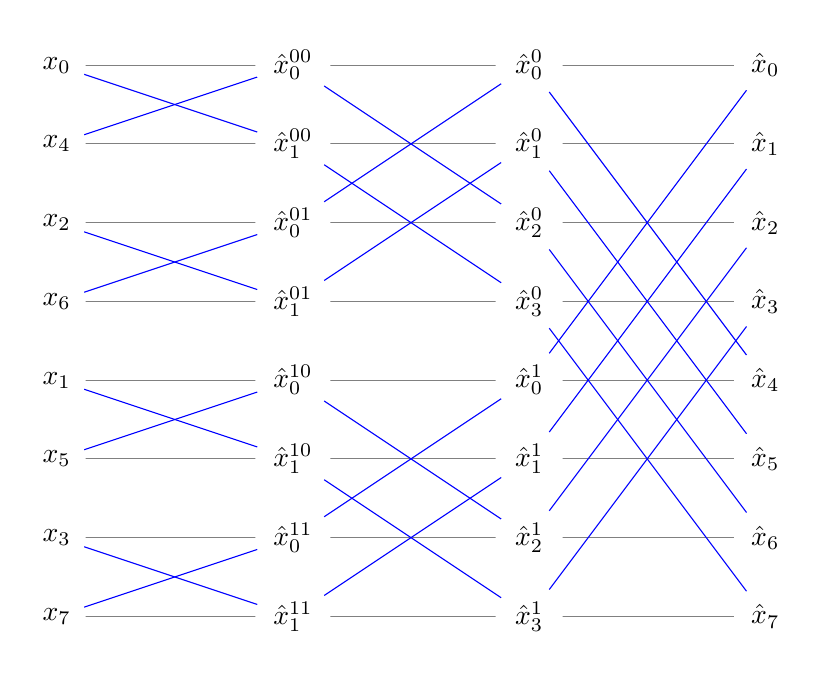
\begin{tikzpicture}[base/.style={gray},cross/.style={draw=blue},
  lab/.style={every node/.style={circle,fill=white}}]
  \foreach \y in {7,6,5,4,3,2,1,0} \draw[base] (0,\y) -- (9,\y);
  \draw[cross] (0,7) -- (3,6) -- (6,4) -- (9,0);
  \draw[cross] (0,6) -- (3,7) -- (6,5) -- (9,1);
  \draw[cross] (0,5) -- (3,4) -- (6,6) -- (9,2);
  \draw[cross] (0,4) -- (3,5) -- (6,7) -- (9,3);
  \draw[cross] (0,3) -- (3,2) -- (6,0) -- (9,4);
  \draw[cross] (0,2) -- (3,3) -- (6,1) -- (9,5);
  \draw[cross] (0,1) -- (3,0) -- (6,2) -- (9,6);
  \draw[cross] (0,0) -- (3,1) -- (6,3) -- (9,7);

  \draw[lab] (0,7) node {$x_0$}
             (0,6) node {$x_4$}
             (0,5) node {$x_2$}
             (0,4) node {$x_6$}
             (0,3) node {$x_1$}
             (0,2) node {$x_5$}
             (0,1) node {$x_3$}
             (0,0) node {$x_7$};
  \draw[lab] (3,7) node {$\hat{x}_0^{00}$}
             (3,6) node {$\hat{x}_1^{00}$}
             (3,5) node {$\hat{x}_0^{01}$}
             (3,4) node {$\hat{x}_1^{01}$}
             (3,3) node {$\hat{x}_0^{10}$}
             (3,2) node {$\hat{x}_1^{10}$}
             (3,1) node {$\hat{x}_0^{11}$}
             (3,0) node {$\hat{x}_1^{11}$};
  \draw[lab] (6,7) node {$\hat{x}_0^{0}$}
             (6,6) node {$\hat{x}_1^{0}$}
             (6,5) node {$\hat{x}_2^{0}$}
             (6,4) node {$\hat{x}_3^{0}$}
             (6,3) node {$\hat{x}_0^{1}$}
             (6,2) node {$\hat{x}_1^{1}$}
             (6,1) node {$\hat{x}_2^{1}$}
             (6,0) node {$\hat{x}_3^{1}$};
  \draw[lab] (9,7) node {$\hat{x}_0$}
             (9,6) node {$\hat{x}_1$}
             (9,5) node {$\hat{x}_2$}
             (9,4) node {$\hat{x}_3$}
             (9,3) node {$\hat{x}_4$}
             (9,2) node {$\hat{x}_5$}
             (9,1) node {$\hat{x}_6$}
             (9,0) node {$\hat{x}_7$};
\end{tikzpicture}\end{center}

The computation proceeds from left to right. The values on the left column
resent a permutation of the input sequence. The superscripts denote
subtransforms, the superscripted ones denote the odd and zeroes the even members
of its parent sequence. Notice that the amount of work and communication
in each stage is linearly proportional to $N$, and that the number of stages grows
with $\log N$.  From this we deduce that the complexity of the computation and
communication is $\mathcal{O}(N \log N)$, which is much more efficient than the
quadratic summation we started this section with. The Cooley-Tukey theorem
obviously holds for the inverse transform, and we conclude therefore that the
long range potential can be evaluated by this method in $\mathcal{O}(N \log N)$
time and communication (the linear computational complexity of evaluating the
convolution in the discrete Fourier basis is asymptotically negligible).

\section{Distributed Implementation}
We have implemented a the discrete Fourier transform in a library suitible for
distributed memory simulations. We assume each processor contains the same size
of data, and that the processors are arranged in a uniform grid. The
implementation supports any number of dimensions (greater than zero). This means
that in each direction, there net dimension of data can be expressed as $PM$,
where $P$ is the number of processors in that direction, and $M$ is the length
of the data array in that direction on each processor. The operation of our
algorithm is as follows (the steps are described in the one dimensional case for
simplicity):
\begin{enumerate}
  \item The data on all processors is rearranged to a $P$ cyclic layout. This
means that the $p$-th processor contains data elements $\{p,P+p,2P+p, \dots
(M-1)P + p\}$.
  \item Each processor performs a serial transform of length $M$ on its data.
This is the inner transform of theorem \ref{thm:CT}.
  \item The data is rearranged by an $M$-cyclic permutation. This results in a
nonuniform distribution of data on each processor (since in general, $P$ does
not divide $M$) but a best effort is made to balance the load on each processor.
  \item Twiddle factors are multiplied onto the data. These are the exponential
terms not part of a Fourier transform in equation \eqref{eqn:cooleyTukey}.
  \item Each processor performs a number of $P$-length serial transforms.
  \item The communication of step three is reversed so that the $p$-th processor
holds data elements from $pM$ to $p(M+1) - 1$ in increasing order.
\end{enumerate}
To evaluate the inverse transform, the same steps are performed in reverse
order with the direction of communication reversed and with the serial
transforms replaced with inverse discrete Fourier transforms. (Actually, the
inverse transform does not account for the factor of $\frac{1}{PM}$ which the
inverse transform should apply. This is to be consistent with the FFTW serial
Fourier transform library, the de facto implementation of the discrete Fourier
transform used in high performance computing.)

The first step is to arrange the data in a $P$-cyclic layout. This is done
because the inner transforms operate on elements spaced $P$ units apart in the
original sequence. If we are performing a recursive application of the
Cooley-Tukey procedure, then we need to further cycle the data according to the
length of the nested transforms. The following schematic shows the proper
ordering (in the lowest level) for a length $12$ transform which is to be
performed by a recursive transform with length sequence $\{3, 2, 2\}$. The first step
separates the data into $3$ groups which are strided $3$ indices apart. The
second and third steps separate each group into two further elements which are
strided two apart. The recursion terminates when we reach a unit length
sequence, which is its own discrete Fourier transform.

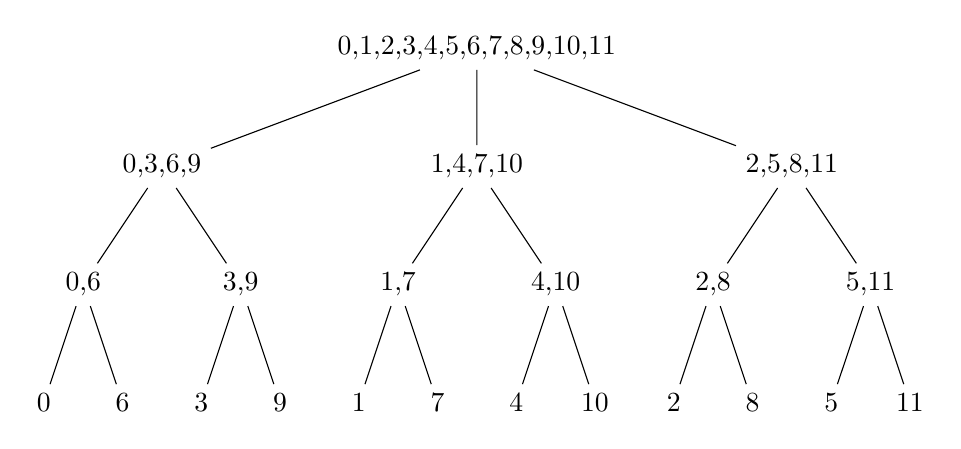
\begin{tikzpicture}[
  level 1/.style={sibling distance=40mm},
  level 2/.style={sibling distance=20mm},
  level 3/.style={sibling distance=10mm}]
  \node {0,1,2,3,4,5,6,7,8,9,10,11}
    child { node {0,3,6,9}
      child { node {0,6} child { node {0} } child { node {6} } }
      child { node {3,9} child { node {3} } child { node {9} } }
    }
    child { node {1,4,7,10}
      child { node {1,7} child { node {1} } child { node {7} } }
      child { node {4,10} child { node {4} } child { node {10} } }
    }
    child { node {2,5,8,11}
      child { node {2,8} child { node {2} } child { node {8} } }
      child { node {5,11} child { node {5} } child { node {11} } }
    };
\end{tikzpicture}

The second step is to perform a serial transform of length $P$. This is
delegated to the highly efficient FFTW library. Internally, it uses a variety of
algorithms\cite{FFTW05} to handle transforms of arbitrary sizes, since the
Cooley-Tukey algorithm is best applied when the length is a product of small
primes. The asymptotic complexity of these algorithms remains $\mathcal{O}(N
\log N)$ so that our earlier complexity assertion remains valid. The FFTW
library is entirely serial, and this step is done on individual processors with
zero communication.

The next step is to perform an $M$-cyclic permutation of the data. The is done
so that the second serial transform can be done on a single processor with no
communication. In the following diagram, we show how we perform a transform of
length $8$ with $2$ processors each holding $4$ units of data:
\begin{center}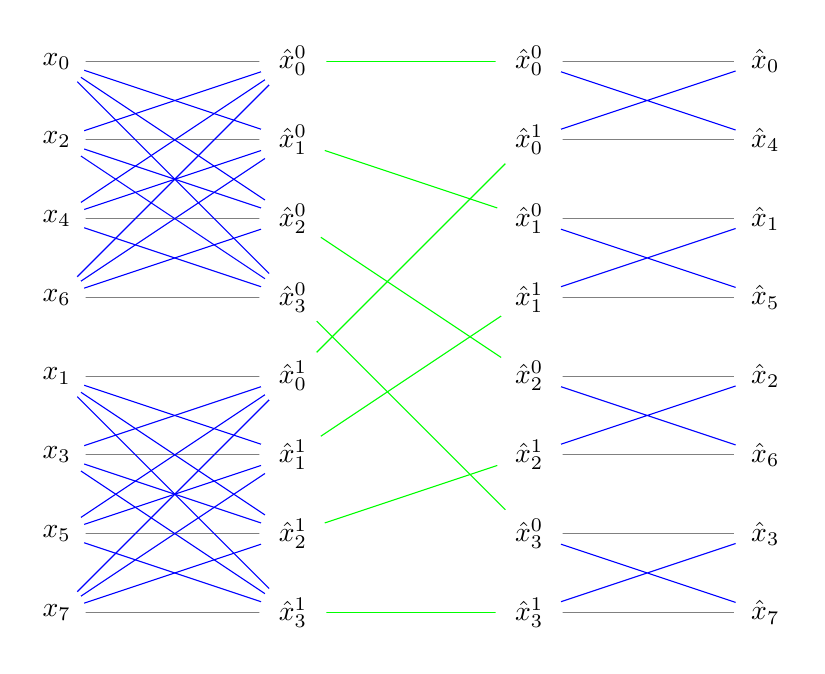
\begin{tikzpicture}[base/.style={gray},cross/.style={draw=blue},
  transp/.style={draw=green},lab/.style={every node/.style={circle,fill=white}}]
  \foreach \y in {7,6,5,4,3,2,1,0} \draw[base] (0,\y) -- (3,\y)
    (6,\y) -- (9,\y);
  \draw[cross] (0,7) -- (3,4) (0,7) -- (3,5) (0,7) -- (3,6);
  \draw[cross] (0,6) -- (3,4) (0,6) -- (3,5) (0,6) -- (3,7);
  \draw[cross] (0,5) -- (3,4) (0,5) -- (3,6) (0,5) -- (3,7);
  \draw[cross] (0,4) -- (3,5) (0,4) -- (3,6) (0,4) -- (3,7);
  \draw[cross] (0,3) -- (3,0) (0,3) -- (3,1) (0,3) -- (3,2);
  \draw[cross] (0,2) -- (3,0) (0,2) -- (3,1) (0,2) -- (3,3);
  \draw[cross] (0,1) -- (3,0) (0,1) -- (3,2) (0,1) -- (3,3);
  \draw[cross] (0,0) -- (3,1) (0,0) -- (3,2) (0,0) -- (3,3);

  \draw[transp] (3,7) -- (6,7);
  \draw[transp] (3,6) -- (6,5);
  \draw[transp] (3,5) -- (6,3);
  \draw[transp] (3,4) -- (6,1);
  \draw[transp] (3,3) -- (6,6);
  \draw[transp] (3,2) -- (6,4);
  \draw[transp] (3,1) -- (6,2);
  \draw[transp] (3,0) -- (6,0);

  \draw[cross] (6,7) -- (9,6) (6,6) -- (9,7);
  \draw[cross] (6,5) -- (9,4) (6,4) -- (9,5);
  \draw[cross] (6,3) -- (9,2) (6,2) -- (9,3);
  \draw[cross] (6,1) -- (9,0) (6,0) -- (9,1);

  \draw[lab] (0,7) node {$x_0$}
             (0,6) node {$x_2$}
             (0,5) node {$x_4$}
             (0,4) node {$x_6$}
             (0,3) node {$x_1$}
             (0,2) node {$x_3$}
             (0,1) node {$x_5$}
             (0,0) node {$x_7$};
  \draw[lab] (3,7) node {$\hat{x}_0^{0}$}
             (3,6) node {$\hat{x}_1^{0}$}
             (3,5) node {$\hat{x}_2^{0}$}
             (3,4) node {$\hat{x}_3^{0}$}
             (3,3) node {$\hat{x}_0^{1}$}
             (3,2) node {$\hat{x}_1^{1}$}
             (3,1) node {$\hat{x}_2^{1}$}
             (3,0) node {$\hat{x}_3^{1}$};
  \draw[lab] (6,7) node {$\hat{x}_0^{0}$}
             (6,6) node {$\hat{x}_0^{1}$}
             (6,5) node {$\hat{x}_1^{0}$}
             (6,4) node {$\hat{x}_1^{1}$}
             (6,3) node {$\hat{x}_2^{0}$}
             (6,2) node {$\hat{x}_2^{1}$}
             (6,1) node {$\hat{x}_3^{0}$}
             (6,0) node {$\hat{x}_3^{1}$};
  \draw[lab] (9,7) node {$\hat{x}_0$}
             (9,6) node {$\hat{x}_4$}
             (9,5) node {$\hat{x}_1$}
             (9,4) node {$\hat{x}_5$}
             (9,3) node {$\hat{x}_2$}
             (9,2) node {$\hat{x}_6$}
             (9,1) node {$\hat{x}_3$}
             (9,0) node {$\hat{x}_7$};
\end{tikzpicture}\end{center}
At the left column, the data has been arranged into a 2-cyclic layout. This
enables the first transform of length 4 to be computed on each processor without
any communication. In the center of the diagram, we rearrange the data by
applying a $4$-cyclic permutation. This enables the outer transforms of length
$2$ to be computed on a single processor. Notice that each processor performs
two second stage computations.

The twiddle factors are applied after the transpose operation, and the second
stage transforms are performed. This leaves the data in a $4$-cyclic permutation
on the processors. Reversing the center communication step in the above diagram
will place the data in ascending order.

\section{Implementation Details}
The preceding high-level overview of the algorithm glossed over the particular
details of the implementation. When we first implemented the code, we first
implemented the naïve algorithm presented in the previous section, and a battery
of tests to verify the correct operation. Optimizations have caused our
implementation to diverge from the simple description provided above. Our
implementation also is able to handle Fourier transforms of vectors in a single
pass.

The previous section describes the parallel transform algorithm in one
dimension. It would be correct to implement multi-dimensional operation by a
sequence of vector-valued transforms in each direction, but this is problematic
for several reasons. The first is that the data is kept in row major format, and
bulk data shuffling would be required to obtain all but the last dimension in a
contiguous vector. This could be addressed by adapting the one dimension routine
to perform multivector transforms with flexible stride parameters, similar to
the guru interface of FFTW. The problem would remain that for a $d$ dimensional
transform, $d$ times as many communications would be required, and this is
inefficient: more data is sent and so more bandwidth and time is wasted, but
there is also a latency cost associated with communication. It is better to
perform fewer, larger communications, thereby minimizing the cost of transfer latency.

Our implementation performs the entire multidimensional transfer in one step,
simultaneously exchanging data in all directions with all other processors. The
first stage communication is implemented using a collective operation,
\texttt{MPI\_Alltoallw} which may be implemented to exploit the network topology
to perform the exchange of data from each node to another as efficiently as
possible. The inner transform is also computed by a multidimensional routine of
FFTW. It would be desirable to extend the interface to accept a similar
interface for arbitrarily looped and strided data similar to the guru interface
of FFTW, the flexibility of this interface proved useful in optimizing the
parallel transform routines and would also be useful in integrating the library
into existing simulations which were developed without our data layout
assumptions in mind.

The second stage communication is not performed using \texttt{MPI\_Alltoallw}.
That routine must wait until the data is received from and sent to all other
processors before completing: it blocks until the operation is completed. We
instead exploit the asynchronous communication facility of MPI to perform the
second stage of communication. The data is requested to be send and received,
but the calls do not block. Instead, we wait for any receive call to complete
and then immediately perform the twiddle factor computations for the data
received from that processor. We then wait for another receive to complete, and
operate on that data. This enables us to partially hide the latency of one stage
of communication by performing useful computation during that period.
This method is not suitable for the first stage of communication since the first
stage transform requires all data be received before the first stage computation
can begin.

There are software engineering considerations which make it undesirable to
modify the first or third stage communication to use non-blocking communication.
The communication and computation of the parallel Fourier routine is wrapped
into a single function, \texttt{fft\_par\_execute\_fwd}, which would need to be
modified to expose more of the internals of the implementation, making it harder
to use. A better idea would be to provide functions to preflight the transform
by queueing asynchronous communication requests for the first stage. The system
could then do some useful work, such as the short range interaction computation,
before calling a function to finish executing the transform, which would first
ensure the previously scheduled operations completed before launching into the
computation. The third stage communication is not even necessary, since if we
are computing the convolution, there is no advantage to having the data in a
block rather than a cyclic layout. The interface should be extended to avoid the
third stage communication and thereby eliminate the communication cost.

To ensure a robust and high-quality implementation, there is a test library to
ensure the correct operation of the library. There are several different
varieties of tests. The first computes a serial transform of a large amount of
data using FFTW, and then performs a parallel transform of the same data. The
two results are checked for consistency by ensuring the corresponding values are
identical (to within a numerical tolerance, currently one part in a million).
There is also a vectorized version of this test. The reverse transform routines
are tested by ensuring that performing a distributed forward transform followed
by a distributed reverse transform yields the original data, there is also a
vectorized version of this test. The parallel routines are checked in one and
two dimensions, the tests should be adapted to run in an arbitrary number of
dimensions. The tests have all been run under the memory profiler Valgrind and
the transforms execute without a single memory leak, read of uninitialized data,
or out of bounds memory access.

The overall usage of the parallel discrete Fourier transform library is inspired
by the FFTW interface. One allocates a plan which encapsulates the transform
paramaters, this plan can then be executed in the forward or backward direction
an arbitrary number of times. The plan structure allows us avoid overhead in the
execution of the transform by caching large memory allocations and persistent
asynchronous communication requests in the plan data. The public interface is
provided in \texttt{fft\_par.h}. The tests give an overview of the usage, and
there has been some work to provide quality documentation in the headers.

The library operates correctly and robustly. We have yet to rigorously test it
in a true distributed memory environment with high communication latency, but
the performance on SMP machines needs to be improved before a more challenging
environment is attempted. We have already described several weaknesses in the
interface which should be addressed in the next iteration of the implementation:
increasing the flexibility of the planner to address non-contiguous storage and
to provide an asynchronous interface to the library.  There is also a need for
design changes under the hood.

The parallel efficiency of the current implementation is very poor, we have
measured a peak efficiency of twenty seven percent on a four processor
two-dimensional transform with a lattice of $1022\times 822$ with a vector
length of one. There are a few design errors which need to be fixed. The
communication routines make elaborate use of MPI's datatype description facility
to transmit from and receive to noncontiguous memory. This was thought to be a
good idea as it would enable the serial transforms to operate on contiguous
memory. In retrospect, it appears to undermine the advantages of asynchronous
communication. The implementation of \texttt{MPI\_Alltoallw} in MPICH2 uses
asynchronous send and receive, and our second stage is explicitly implemented
using asynchronous communication. These are implemented by forking threads to
receive the data in the background using blocking operations and write it to its
destination outside the computational master thread or to read the data from its
location and send it using blocking operations. It is easy (with hindsight) to
see that our decision to scatter data from multiple processors into one memory
region is a disaster: the receiving threads end up battling for control of the
cache lines, and this wastes memory bandwidth. In the second stage
communication, the master thread which is applying twiddle factors also joins
the battle. The effect of this memory contention is to increase the latency of
every transmission and reception and to degrade the efficiency of computation.
We believe this can be rectified by having the processors send and receive to
contiguous memory and to have the serial transform deal with the noncontiguous
data. We have already used the guru interface of FFTW to do this for our second
serial transform, it should be sufficiently flexible for this purpose as well.

\bibliography{magnetics,fourier,fftw}
\end{document}
